\documentclass[12pt]{article}
\textwidth 16.5cm
\textheight 23.5cm
\oddsidemargin 0pt
\topmargin -2cm
% \usepackage{epsf}

% Writing maths
\usepackage{
    amsmath, % aligns, equations, etc.
    amsfonts, % blackboard bold, etc.
    bbm, % blackboard bold for numbers.
}

% Figures
\usepackage{graphicx}

% References
\usepackage{hyperref}

% References 
\usepackage{natbib}
\bibliographystyle{natbib}
\setcitestyle{authoryear, open={(},close={)}}

% Inline comments from Jacob and Bella
\usepackage{xcolor}
\usepackage[draft,inline,nomargin,index]{fixme}
\fxsetup{theme=color,mode=multiuser}
\FXRegisterAuthor{jb}{ajb}{\color{blue} JB}
\FXRegisterAuthor{bd}{abd}{\color{red} BD}

\title{Simulations of Immigration Queues at Edinburgh Airport: Tech Setup}
 \author{Jacob R. Bradley
 \\ \emph{School of Mathematics, University of Edinburgh}}

\begin{document}
\maketitle

\section{Introduction}
This document contains descriptions of how GitHub, RStudio, Overleaf, and Zotero interact for a (hopefully) seamless and ultra-efficient competition-smashing workflow!

\section{Methods}
\subsection{GitHub}
The code for this project is held in a \href{https://github.com/cobrbra/immigration_queue_simulation_edinburgh_airport}{GitHub repository}. This stores and tracks the history of all the data, code, and docs associated with the project, but shouldn't be used directly for editing anything aside from in an emergency! Instead, coding should be done in RStudio and writing should be done in Overleaf. In GitHub, you can see the entire project folder layout (Figure~\ref{fig:github_overview}).

\begin{figure}[htbp]
    \centering
    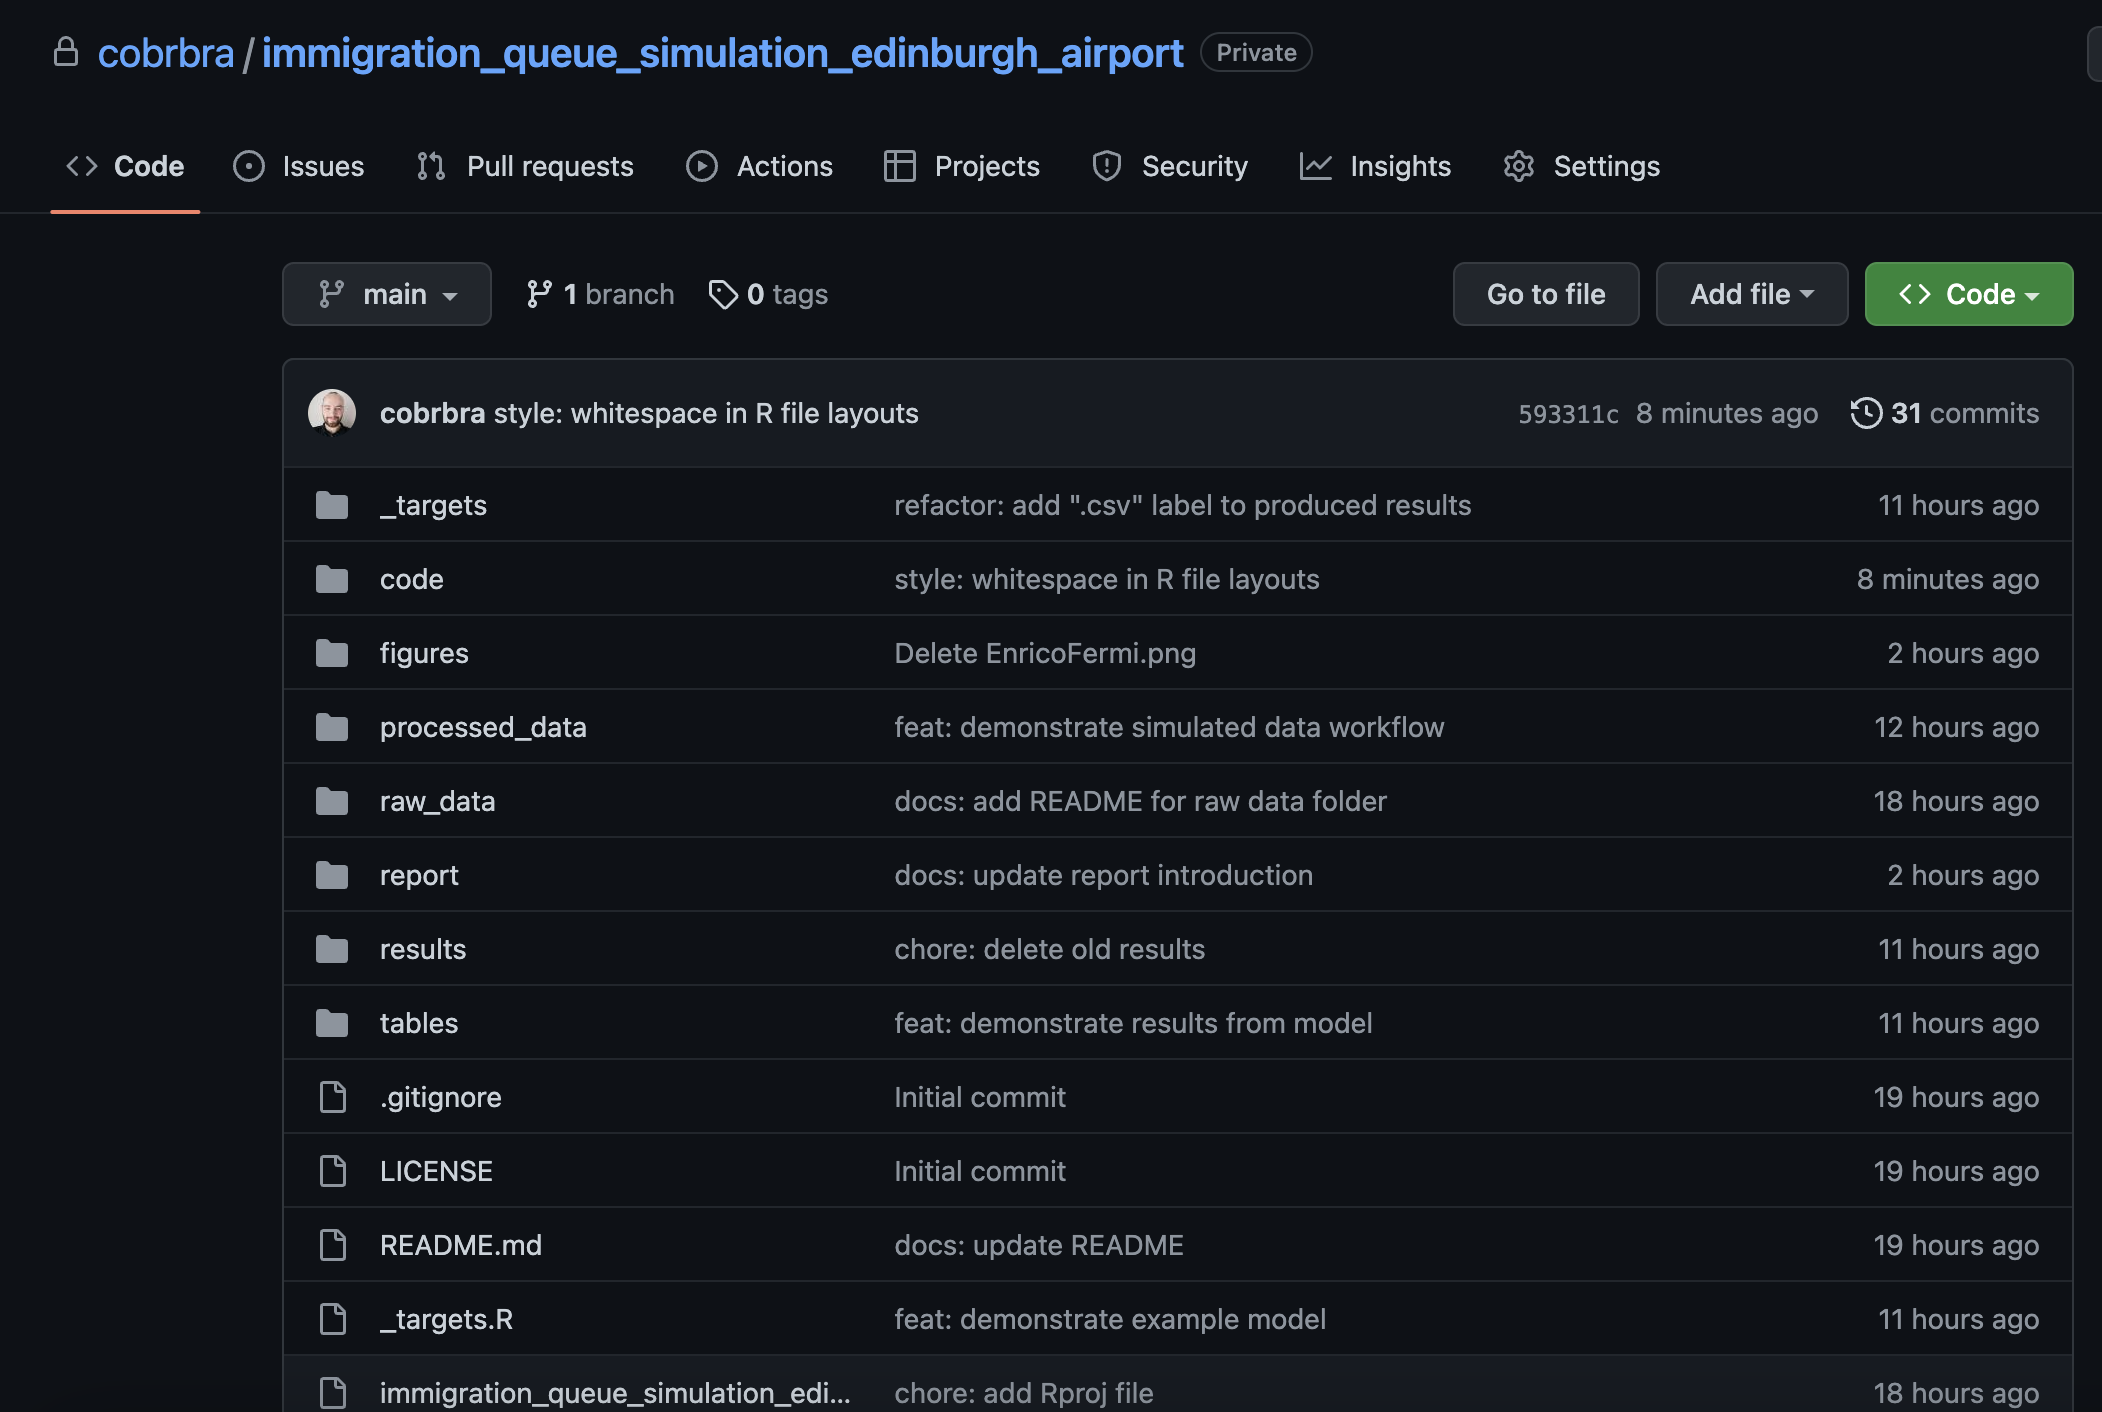
\includegraphics[width=4in]{figures/github_overview.png}
    \caption{GitHub view of project folder.}
    \label{fig:github_overview}
\end{figure}

The ``Code'' tab will be useful for syncing GitHub with RStudio (see below). Syncing with Overleaf should already have been done from here.


\subsection{RStudio}
RStudio will be where (separately) we each do coding for the project. We'll each have our own ``local'' copy, which will be linked to GitHub, where the ``main'' copy will be stored. When we want to share some of the changes we've made, we'll ``commit'' them (i.e. select which changes are ready to be shared) and then ``push'' them. When we want to update with other changes that have been made, we'll ``pull'' these from the main version in GitHub. 

To get started, we'll need to set up the repository as a project in RStudio. You can do this with \texttt{File} $\rightarrow$ \texttt{New Project} $\rightarrow$ \texttt{Version Control} $\rightarrow$ \texttt{Git}. You should then enter the repository URL \href{git@github.com:cobrbra/immigration_queue_simulation_edinburgh_airport.git}{git@github.com:cobrbra/immigration\textunderscore queue\textunderscore simulation\textunderscore edinburgh\textunderscore airport.git} (we'll need to do some faffing around with ssh keys i.e. permissions, but that'll be a one-time thing). You should put the repository name (not including my GitHub handle) as the project name and choose where in your system you want it all stored (see Figure~\ref{fig:rstudio_new_project}). 

\begin{figure}[htbp]
    \centering
    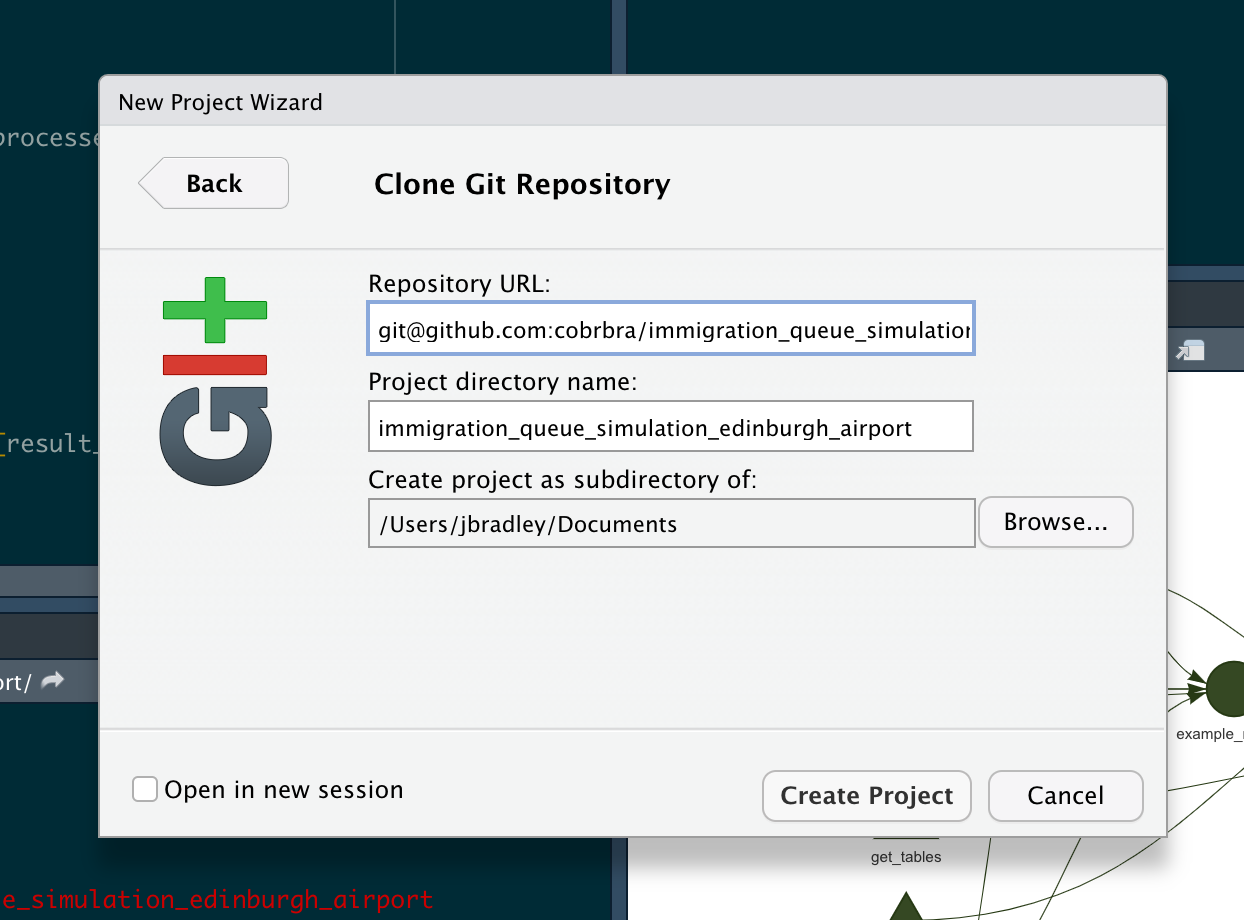
\includegraphics[width=4in]{figures/rstudio_new_project.png}
    \caption{Creating a new project from Git in RStudio.}
    \label{fig:rstudio_new_project}
\end{figure}

Once the project is made, you can begin making changes to it (make sure that the project is open in RStudio before you do. If it's loaded the project name will appear at the top of the RStudio window. If it isn't, you can go \texttt{File} $\rightarrow$ \texttt{Open Project} then select). You can now make edits to any file as you would for normal work. Once you've done, it's time to use the \texttt{Commit}, \texttt{Pull}, and \texttt{Push} buttons available in the Git panel on the top right hand of RStudio (Figure~\ref{fig:rstudio_git_panel}).

\begin{figure}[htbp]
    \centering
    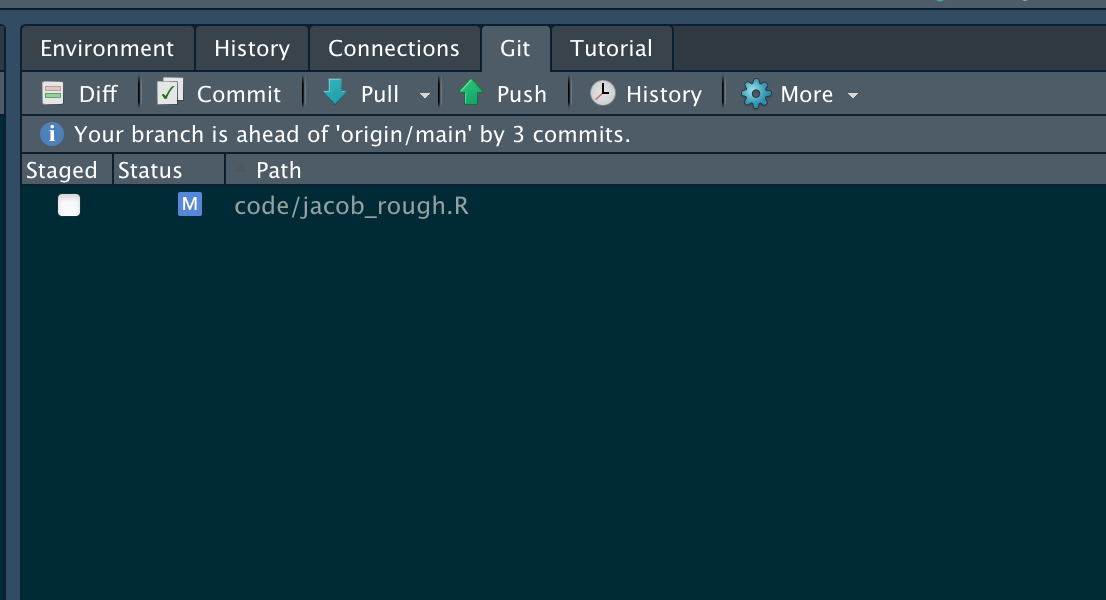
\includegraphics[width=4in]{figures/rstudio_git_panel.png}
    \caption{Creating a new project from Git in RStudio.}
    \label{fig:rstudio_git_panel}
\end{figure}

\subsubsection{Commits}
When you've made some edits than form a coherent piece of work, it's time to commit those edits. This doesn't do anything yet, you're just checking them in as work done and `staging' them as ready to be pushed (remember, pushing means sending your local copy up to be added to the main version stored on GitHub). You can see in Figure~\ref{fig:rstudio_git_panel} that my local version (my `branch') is ahead by three commits of the main branch on GitHub. That's fine, but in general it's good practice not to let this list grow too long, or we'll risk there being too many conflicting changes for Git to know how to reconcile. 

I've made a minor change to the file ``code/jacob\_rough.R''. To evaluate whether or not I want to commit it, I'm going to press the big ``Commit'' button, where I'll be able to see the changes I've made laid out. I can choose files which to add by ticking the check boxes next to them, then write a commit message and submit the commit. Commit messages should be short, and meaningfully describe the changes made. If you can't think of a good commit message, consider making a smaller commit!

\subsubsection{Pushes and Pulls}
Once you've made a commit, it's time to push it (i.e. give it to the main version on GitHub). Before you do that, though, I'd always recommend clicking Pull first, so that you can get up to date with the latest edits to the main version. In general, these will be integrated seamlessly with your changes, but if Git gets confused then it throws a warning and makes us do some extra stuff to reconcile our working versions.

\subsection{Overleaf}
I've associated this Overleaf project with the GitHub repository for this project. We still need to do pushes and pulls backwards and forwards (Overleaf automatically commits all changes for us). You can do this via \texttt{Menu} $\rightarrow$ \texttt{GitHub}. In general as we're using Overleaf for writing and RStudio for coding, the pushes made my Overleaf should be fairly conflict free. The main use case for this is if we've generated figures/tables with code, having them automatically available in Overleaf to use, rather than having to copy manually and keep a track of all latest versions.
\subsection{Zotero}
\subsection{Targets}

% \section{Results}

% \begin{figure}[htbp]
%     \centering
%     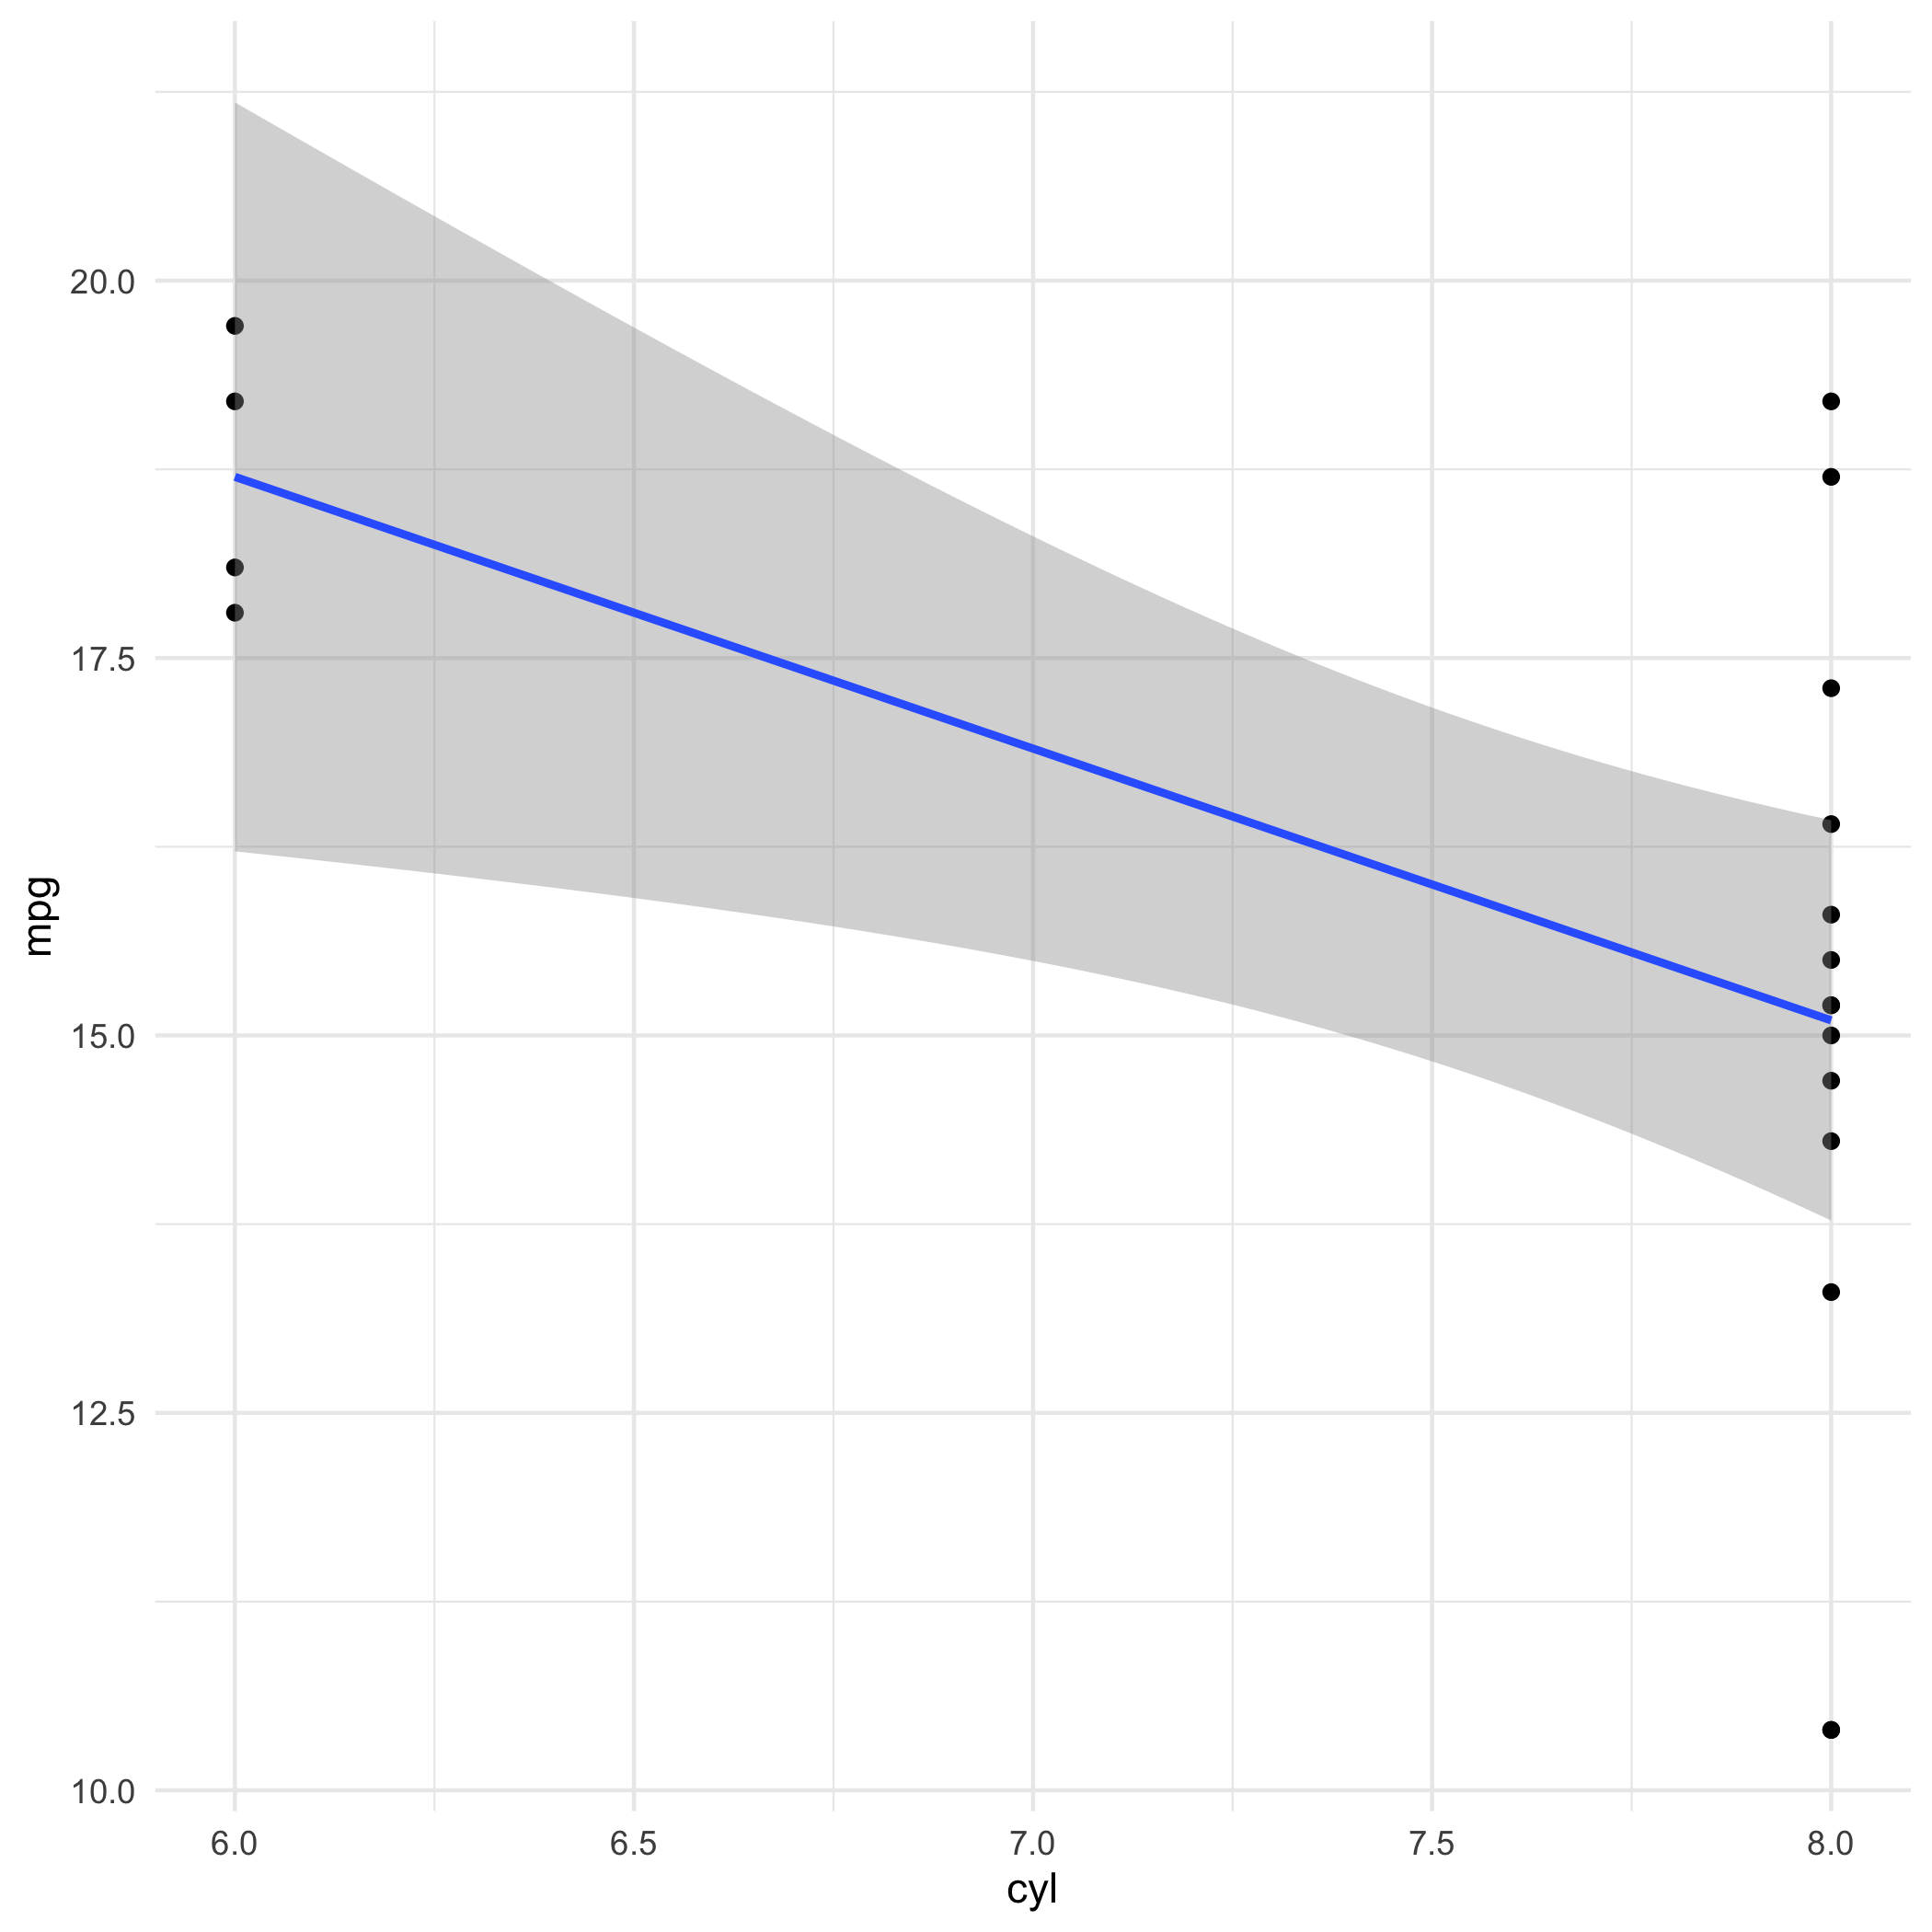
\includegraphics[width=4in]{figures/mt_cars_summary.png}
%     \caption{Example figure generated from mtcars workflow.}
%     \label{fig:mtcars}
% \end{figure}

% \begin{figure}[htbp]
%     \centering
%     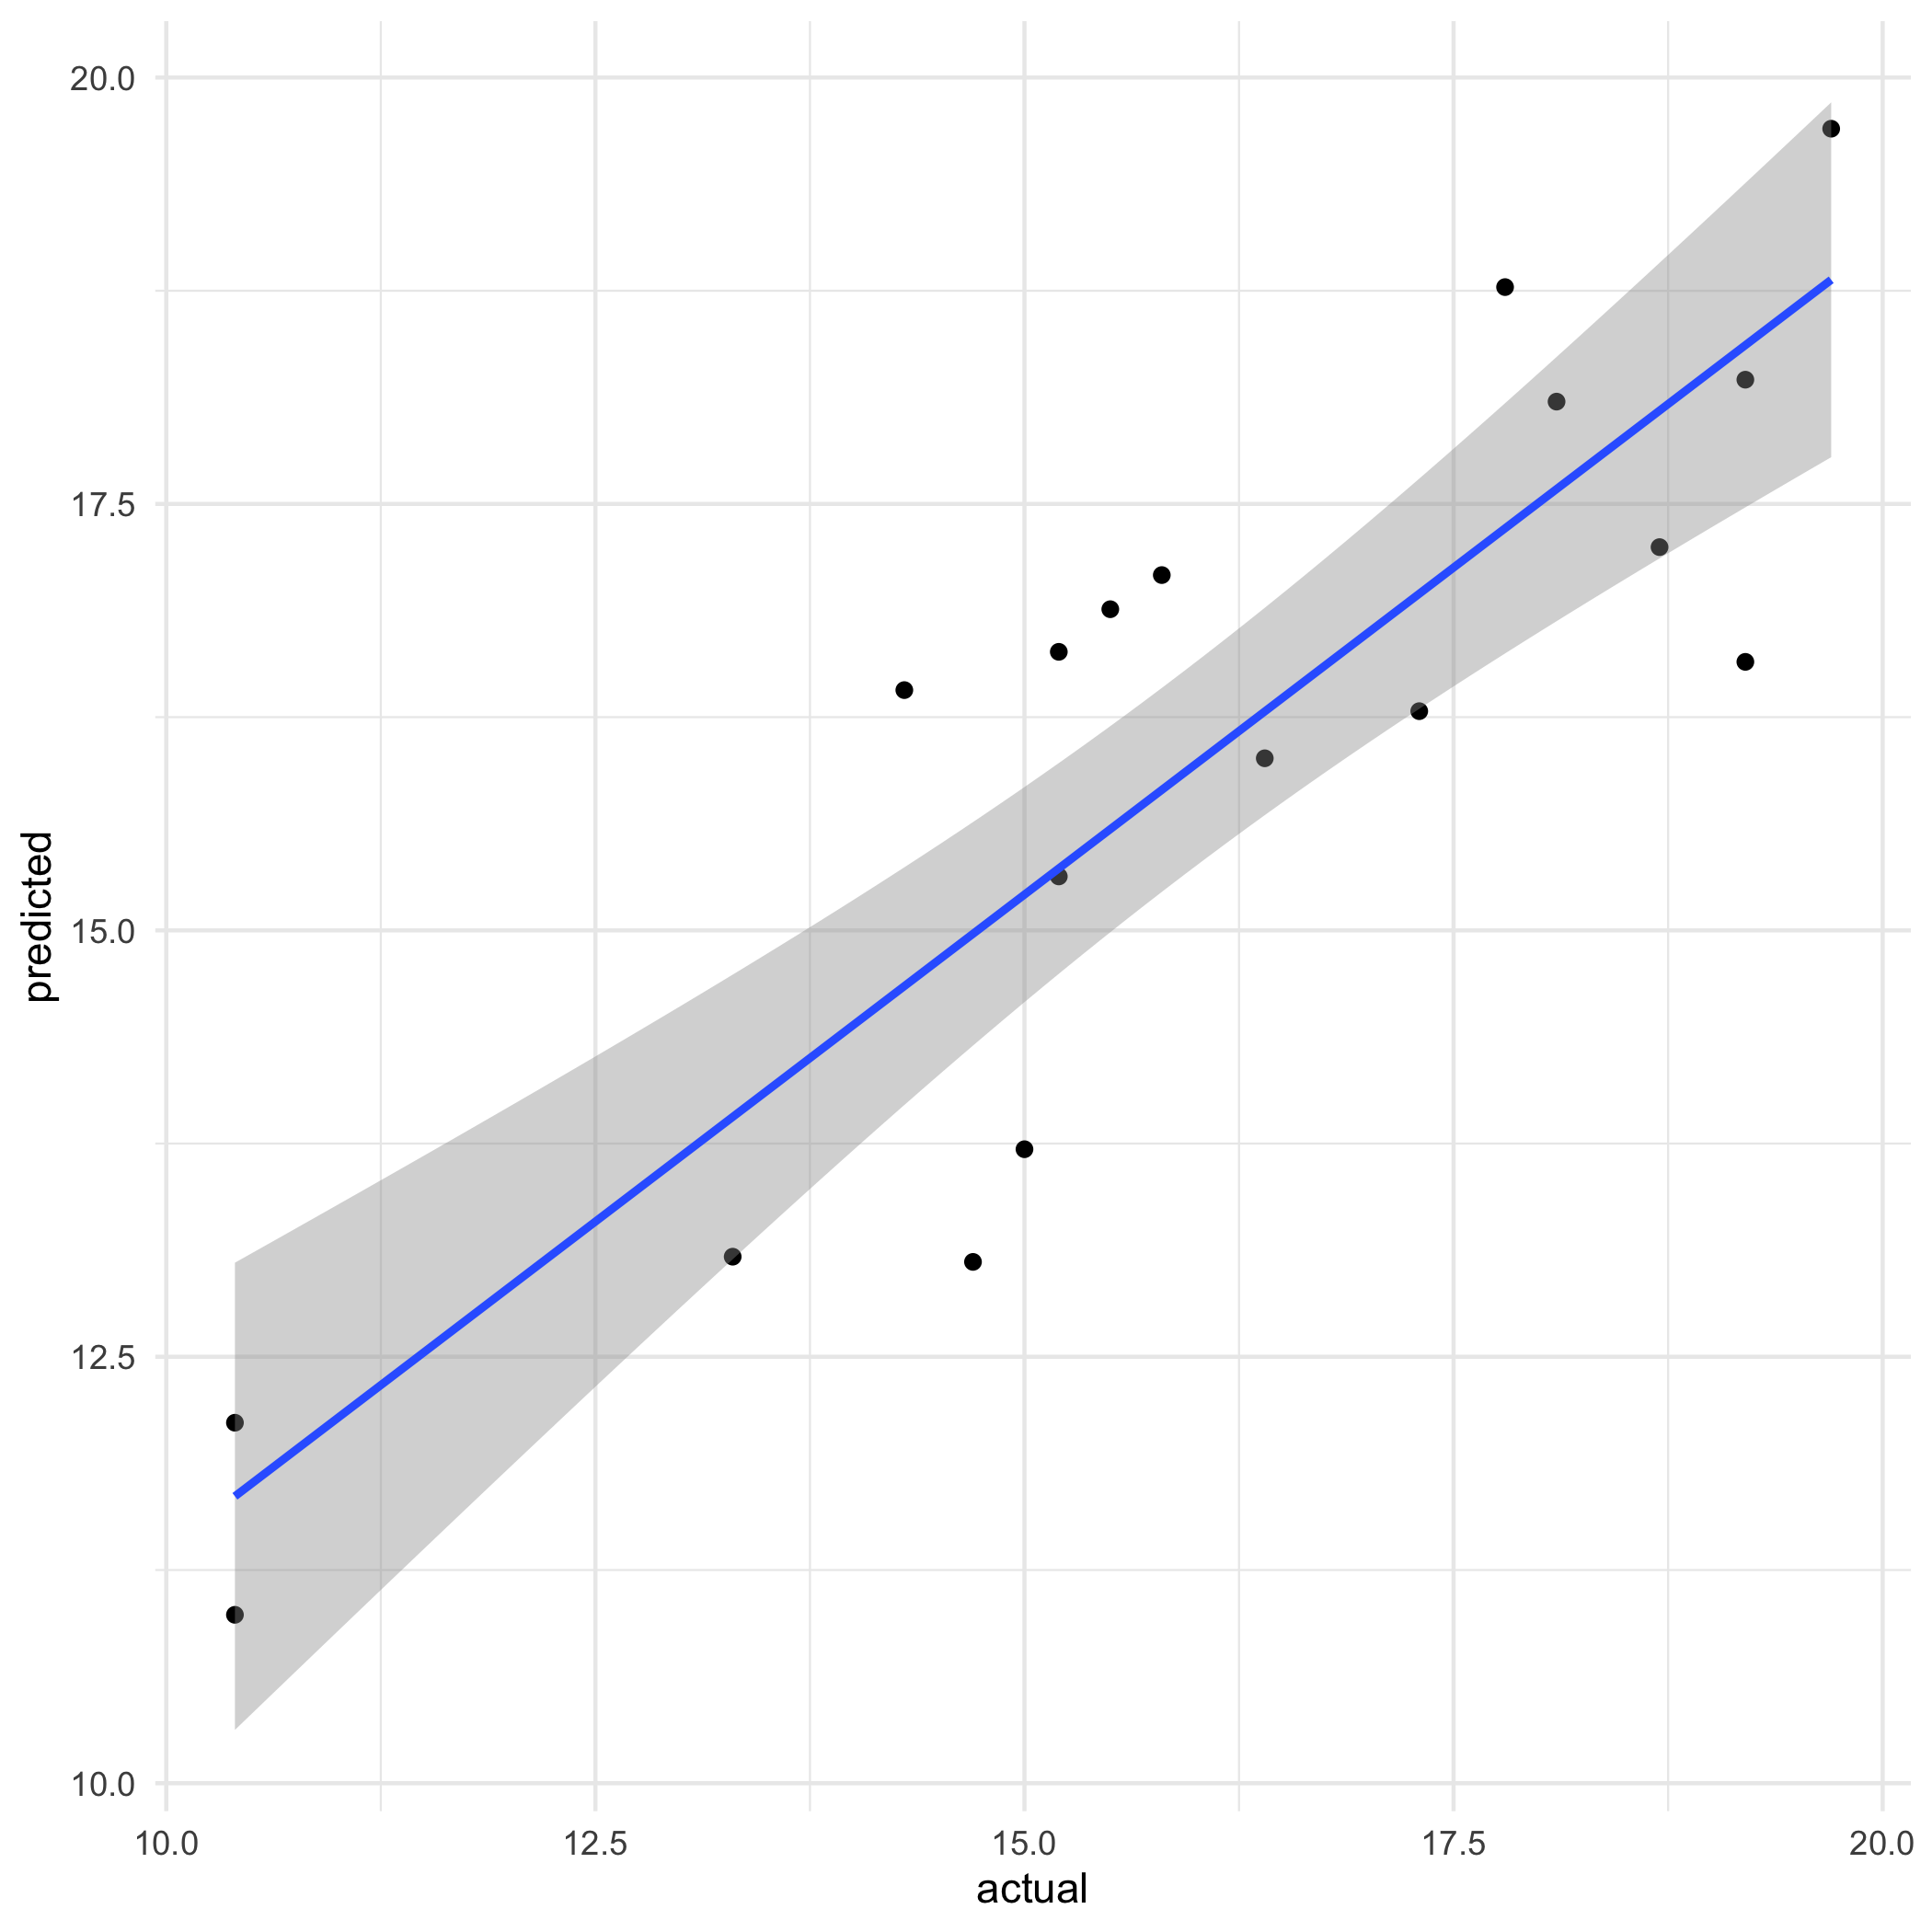
\includegraphics[width=4in]{figures/mpg_model_actual_vs_predicted.png}
%     \caption{Example figure generated from a model of mtcars data.}
%     \label{fig:mtcars_model}
% \end{figure}

% % latex table generated in R 4.2.2 by xtable 1.8-4 package
% Wed Feb 22 17:14:53 2023
\begin{table}[ht]
\centering
\begin{tabular}{rrrrrrrrrrrr}
  \hline
 & mpg & cyl & disp & hp & drat & wt & qsec & vs & am & gear & carb \\ 
  \hline
1 & 18.70 & 8.00 & 360.00 & 175.00 & 3.15 & 3.44 & 17.02 & 0.00 & 0.00 & 3.00 & 2.00 \\ 
  2 & 18.10 & 6.00 & 225.00 & 105.00 & 2.76 & 3.46 & 20.22 & 1.00 & 0.00 & 3.00 & 1.00 \\ 
  3 & 14.30 & 8.00 & 360.00 & 245.00 & 3.21 & 3.57 & 15.84 & 0.00 & 0.00 & 3.00 & 4.00 \\ 
  4 & 19.20 & 6.00 & 167.60 & 123.00 & 3.92 & 3.44 & 18.30 & 1.00 & 0.00 & 4.00 & 4.00 \\ 
  5 & 17.80 & 6.00 & 167.60 & 123.00 & 3.92 & 3.44 & 18.90 & 1.00 & 0.00 & 4.00 & 4.00 \\ 
  6 & 16.40 & 8.00 & 275.80 & 180.00 & 3.07 & 4.07 & 17.40 & 0.00 & 0.00 & 3.00 & 3.00 \\ 
  7 & 17.30 & 8.00 & 275.80 & 180.00 & 3.07 & 3.73 & 17.60 & 0.00 & 0.00 & 3.00 & 3.00 \\ 
  8 & 15.20 & 8.00 & 275.80 & 180.00 & 3.07 & 3.78 & 18.00 & 0.00 & 0.00 & 3.00 & 3.00 \\ 
  9 & 10.40 & 8.00 & 472.00 & 205.00 & 2.93 & 5.25 & 17.98 & 0.00 & 0.00 & 3.00 & 4.00 \\ 
  10 & 10.40 & 8.00 & 460.00 & 215.00 & 3.00 & 5.42 & 17.82 & 0.00 & 0.00 & 3.00 & 4.00 \\ 
  11 & 14.70 & 8.00 & 440.00 & 230.00 & 3.23 & 5.34 & 17.42 & 0.00 & 0.00 & 3.00 & 4.00 \\ 
  12 & 15.50 & 8.00 & 318.00 & 150.00 & 2.76 & 3.52 & 16.87 & 0.00 & 0.00 & 3.00 & 2.00 \\ 
  13 & 15.20 & 8.00 & 304.00 & 150.00 & 3.15 & 3.44 & 17.30 & 0.00 & 0.00 & 3.00 & 2.00 \\ 
  14 & 13.30 & 8.00 & 350.00 & 245.00 & 3.73 & 3.84 & 15.41 & 0.00 & 0.00 & 3.00 & 4.00 \\ 
  15 & 19.20 & 8.00 & 400.00 & 175.00 & 3.08 & 3.85 & 17.05 & 0.00 & 0.00 & 3.00 & 2.00 \\ 
  16 & 15.80 & 8.00 & 351.00 & 264.00 & 4.22 & 3.17 & 14.50 & 0.00 & 1.00 & 5.00 & 4.00 \\ 
  17 & 19.70 & 6.00 & 145.00 & 175.00 & 3.62 & 2.77 & 15.50 & 0.00 & 1.00 & 5.00 & 6.00 \\ 
  18 & 15.00 & 8.00 & 301.00 & 335.00 & 3.54 & 3.57 & 14.60 & 0.00 & 1.00 & 5.00 & 8.00 \\ 
   \hline
\end{tabular}
\caption{MTCars dataset restricted to observations with $<20$ miles per gallon \label{tab:mtcars_full}} 
\end{table}


% \section{Discussion}
% \section{Conclusion}
% \bibliography{references.bib}
\end{document}